\part{AMQP}


\chapter{Overview}

\section{Queue}

队列(Queue)又称先进先出表(First In First Out),即先进入队列的元素,先从队列中取出。加入元素的一头叫“队头”,取出元素的一头叫“队尾”。



消息队列可以很好地异步处理数据传送和存储,如果有需要频繁地向数据库中插入数据、频繁地向搜索引擎提交数据的应用场景,就可以采取消息队列来异步插入。



另外,还可以将较慢的处理逻辑或者有并发数量限制的处理逻辑,通过消息队列放在后台处理,例如FLV视频转换、发送手机短信或发送电子邮件等。




\subsection{AMQP}



AMQP(Advanced Message Queuing Protocol)的目标是成为所有的消息中间件互操作的标准协议,其本质是一个功能丰富的消息队列协议。






AMQP的最初设计者iMatix公司的首席执行官Pieter Hintjens宣布iMatix将退出AMQP工作组,而且更简单和更快的的ZeroMQ将不支持可能发布的AMQP/1.0。


和AMQP相似的消息队列协议还有STOMP、XMPP、MQTT和ActiveMQ等,而且不同消息队列往往工作在不同的通信阶段,例如:

\begin{compactitem}
\item AMQP和STOMP和HTTP协议层级相同;
\item MQTT和TCP/IP协议的层级相同。
\end{compactitem}


亚马逊SQS(Amazon Simple Queue Service)使用HTTP协议来提供消息队列,这样用户就可以使用请求/响应(request-response)语义的协议来异步地操作消息队列。





\subsection{STOMP}


STOMP(Streaming Text Oriented Messaging Protocol)是一个简单的基于文本的消息协议。



\subsection{MQTT}

MQTT(MQ Telemetry Transport)是一个专注于嵌入式设备的轻量级的消息队列协议。


\subsection{ZeroMQ}

\section{Message Passing}

UNIX通过将链表的数组保存为消息队列来实现消息传递。 每个消息队列由其在数组中的索引标识,并且具有唯一的描述符。 给定的索引可以具有多个可能的描述符,UNIX提供了访问消息传递功能的标准功能。

\subsection{msgget()}


msgget()系统调用使用键作为参数,并返回具有匹配键的队列的描述符(如果存在)。 如果它不存在,并且IPC\_CREAT标志被设置,它使用给定的键来产生新的消息队列并返回其描述符。


\subsection{msgrcv()}

msgrcv()用于从给定队列描述符接收消息。 调用者进程必须具有队列的读取权限,而且它有两种类型:

\begin{compactitem}
\item 如果msgrcv()找不到请求的消息类型就阻塞接收并将使子进程睡眠,直到另一个消息被发布在队列中,然后唤醒以再次检查。
\item 非阻塞接收立即返回到调用者,并说明接收失败。
\end{compactitem}

\subsection{msgctl()}

msgctl()用于更改消息队列参数(例如所有者),而且最重要的是,它通过传递IPC\_RMID标志来删除消息队列。 

消息队列只能由其创建者,所有者或超级用户删除。


\section{Message Queue}


消息队列最初是一种进程间通信或同一进程的不同线程间的通信方式,软件队列通常用来处理一系列来自用户的输入,组通信系统可以实现和消息队列类似的功能。

消息队列非常独特,因为两个进程不必同时存在,即一个进程可以发送一个消息并退出,而该消息可以在数天后才被另一个进程获得。

消息队列本身是异步的,它允许接收者在消息发送很长时间后再取回消息,这和大多数通信协议是不同的。例如,WWW中使用的HTTP协议(HTTP/2之前)是同步的,因为客户端在发出请求后必须等待服务器回应。

很多情况下,用户需要异步的通信协议。比如,一个进程通知另一个进程发生了一个事件,但不需要等待回应,不过消息队列的异步特点也造成了一个缺点,就是接收者必须轮询消息队列才能收到最近的消息。

\begin{compactitem}
\item 和信号相比,消息队列能够传递更多的信息;
\item 与管道相比,消息队列提供了有格式的数据;
\item 和信号和管道相比,消息队列仍然有大小限制。
\end{compactitem}

消息队列通常都提供了异步的通信协议,每一个队列中的记录包含了详细说明的数据(例如发生的时间、输入设备的种类以及特定的输入参数等)。换句话说,消息的发送者和接收者不需要同时与消息队列互交,消息会保存在队列中,直到接收者取回它。

例如,Windows系统通过某些形式(通常是事件的时间或是重要性的顺序)的事件队列来保存用户触发的事件,并且由系统把每个事件从事件队列中传递给目标应用程序。

在消息队列的实现中,消息队列通常保存在链表结构中并提供有格式的字节流,拥有权限的进程可以向消息队列中写入或读取消息。

消息队列通常使用发布/订阅(publisher/subscriber)模式,而且其典型应用是作为基于服务的中间件系统组成的一部分,大多数消息系统(例如JMS(Java Message Service))都在其提供的API中同时支持发布/订阅模式和消息队列。

消息队列的开源实现包括Apache ActiveMQ、Apache Qpid、Apache Kafka、Beanstalkd、IBM MQ、JBoss Messaging、JORAM、RabbitMQ、Sun Open Message Queue、Tarantool和HTTPSQS等。

消息队列除了可以作为不同线程或进程间的缓冲外,还可以通过消息队列当前消息数量来检测接收线程或进程性能是否有问题。

\chapter{ActiveMQ}





\chapter{RabbitMQ}

RabbitMQ是一个实现了AMQP协议的开源message broker软件(或基于消息的中间件(message-oriented middleware)),其中RabbitMQ服务器是一个基于Open Telecom Platform框架并使用Erlang语言来管理集群和失效转移的实现,RabbitMQ客户端可以使用大多数编程语言实现。


下面的示例使用Python通过RabbitMQ消息队列来发送和接收消息。

\section{Sending}

下面的示例创建一个连接并且在确认消息队列存在后就发送一条消息,然后关闭连接。


\begin{lstlisting}[language=Python]
#! /usr/bin/env python
import pika
connection = pika.BlockingConnection(pika.ConnectionParameters(host='localhost'))
channel = connection.channel()
channel.queue_declare(queue='hello')
channel.basic_publish(exchange='',routing_key='hello',body='Hello world!')
print(" [x] Sent 'Hello world!'")
connection.close()
\end{lstlisting}

\section{Receiving}

下面的示例从消息队列中接收消息并且在屏幕上把消息打印出来。


\begin{lstlisting}[language=Python]
#! /usr/bin/env python
import pika
connection = pika.BlockingConnection(pika.ConnectionParameters(host='localhost'))
channel = connection.channel()
channel.queue_declare(queue='hello')
print(' [*] Wating for messages. To exit press CTRL+C')
def callback(ch,method,properties,body):
   print(" [x] Received %r" % body)
channel.basic_consume(callback,queue='hello',no_ack=True)
channel.start_consuming()
\end{lstlisting}


\chapter{HTTPSQS}


HTTPSQS(HTTP Simple Queue Service)是一款基于 HTTP GET/POST 协议的轻量级开源简单消息队列服务,使用 Tokyo Cabinet 的 B+Tree Key/Value 数据库来做数据的持久化存储。

HTTPSQS 具有以下特征:

\begin{compactitem}
\item 基于 HTTP GET/POST 协议,支持HTTP协议的编程语言均可调用;
\item 执行速度非常快,入队列、出队列速度超过10000次/秒;
\item 支持上万的高并发连接数,可以解决C10K问题;
\item 支持多队列;
\item 单个队列支持的最大队列数量最高可达10亿条;
\item 低内存消耗,海量数据存储,存储数十GB的数据只需不到100MB的物理内存缓冲区;
\item 可以在不停止服务的情况下便捷地修改单个队列的最大队列数量;
\item 可以实时查看队列状态(入队列位置、出队列位置、未读队列数量、最大队列数量);
\item 可以查看指定队列ID(队列点)的内容,包括未出、已出的队列内容;
\item 查看队列内容时,支持多字符集编码;
\end{compactitem}


采用Apache ab命令进行压力测试HTTPSQS,开启10个线程,放入10万条文本数据(每条512字节)到队列中:

\begin{compactitem}
\item 使用HTTP Keep-Alive时:23018 requests/sec
\item 关闭HTTP Keep-Alive时:11840 requests/sec
\end{compactitem}

采用Apache ab命令进行压力测试,开启10个线程,从队列中取出10万条文本数据(每条512字节):

\begin{compactitem}
\item 使用HTTP Keep-Alive时:25982 requests/sec
\item 关闭HTTP Keep-Alive时:13294 requests/sec
\end{compactitem}

在金山游戏官网的生产环境中,新闻、论坛帖子、客服公告、SNS社区等发生的增、删、改操作,文本内容实时写入HTTPSQS队列,全站搜索引擎增量索引准实时(1分钟内)更新的数据源取自HTTPSQS,而且来自支持Web服务器的入队列操作和来自命令行脚本的批量入、出队列操作。


\begin{compactenum}
\item 金山通行证(https://my.xoyo.com)

\begin{compactitem}
\item 队列应用类型:手机短信上行、手机短信下发、邮件下发
\item 队列应用要求:稳定性高,存储数据量大
\item 队列部署结构:一主、一备两台 HTTPSQS 热备模式
\end{compactitem}

\item 金山用户行为分析系统(http://kbi.xoyo.com)

\begin{compactitem}
\item 队列应用类型:用户鼠标点击、访问URL原始数据采集
\item 队列应用要求:并发性能高,存储数据量大
\item 队列部署结构:多台 HTTPSQS 应用层哈希分布式模式
\end{compactitem}

\item 金山网络游戏运营平台 KingEyes

\begin{compactitem}
\item 队列应用类型:用户操作日志记录
\end{compactitem}

\item 金山逍遥网站内搜索

\begin{compactitem}
\item 队列应用类型:索引准实时更新。
\end{compactitem}

\item 金山逍遥网全站通用评论系统

\begin{compactitem}
\item 队列应用类型:评论发表
\end{compactitem}

\item 金山《剑侠情缘》电视连续剧四大角色人物选秀活动(http://zt.xoyo.com/haixuan/)

\begin{compactitem}
\item 队列应用类型:用户上传的照片异步裁剪、缩放处理
\end{compactitem}

\item 新浪邮箱(http://mail.sina.com.cn)

\begin{compactitem}
\item 队列应用类型:用户登陆日志记录
\end{compactitem}
  
\end{compactenum}



\begin{lstlisting}[language=bash]
# ulimit -SHn 65535

$ wget http://httpsqs.googlecode.com/files/libevent-2.0.12-stable.tar.gz
$ tar zxvf libevent-2.0.12-stable.tar.gz
$ cd libevent-2.0.12-stable/
$ ./configure --prefix=/usr/local/libevent-2.0.12-stable/
$ make
# make install
$ cd ../

$ wget http://httpsqs.googlecode.com/files/tokyocabinet-1.4.47.tar.gz
$ tar zxvf tokyocabinet-1.4.47.tar.gz
$ cd tokyocabinet-1.4.47/
$ ./configure --prefix=/usr/local/tokyocabinet-1.4.47/
# ./configure --enable-off64 --prefix=/usr/local/tokyocabinet-1.4.47/
$ make
# make install
$ cd ../

$ wget http://httpsqs.googlecode.com/files/httpsqs-1.7.tar.gz
$ tar zxvf httpsqs-1.7.tar.gz
$ cd httpsqs-1.7/
$ make
# make install
$ cd ../
\end{lstlisting}

在32位Linux操作系统上编译Tokyo cabinet时需要使用\texttt{./configure -\/-enable-off64}代替./configure,可以使数据库文件突破2GB的限制。


\begin{lstlisting}[language=Python]
# httpsqs -h
-l <ip_addr> 监听的IP地址,默认值为 0.0.0.0 
-p <num> 监听的TCP端口(默认值:1218)
-x <path> 数据库目录,目录不存在会自动创建(例如:/opt/httpsqs/data)
-t <second> HTTP请求的超时时间(默认值:3)
-s <second> 同步内存缓冲区内容到磁盘的间隔秒数(默认值:5)
-c <num> 内存中缓存的最大非叶子节点数(默认值:1024)
-m <size> 数据库内存缓存大小,单位:MB(默认值:100)
-i <file> 保存进程PID到文件中(默认值:/tmp/httpsqs.pid)
-a <auth> 访问HTTPSQS的验证密码(例如:mypass123)
-d 以守护进程运行
-h 显示这个帮助
\end{lstlisting}




\begin{lstlisting}[language=bash]
$ ulimit -SHn 65535 
# httpsqs -d -p 1218 -x /data0/queue
\end{lstlisting}

使用命令“killall httpsqs”、“pkill httpsqs”和“kill `cat /tmp/httpsqs.pid`”来停止httpsqs,禁止使用命令“pkill -9 httpsqs”和“kill -9  httpsqs的进程ID”来结束httpsqs,否则内存中尚未保存到磁盘的数据将会丢失。


\section{Put}


入队列(将文本消息放入队列)

HTTP GET 协议(以curl命令为例)

\begin{lstlisting}[language=bash]
$ curl "http://host:port/?name=your_queue_name&opt=put&data=经过URL编码的文本消息&auth=mypass123"
\end{lstlisting}


HTTP POST 协议(以curl命令为例):

\begin{lstlisting}[language=Python]
$ curl -d "经过URL编码的文本消息" "http://host:port/?name=your_queue_name&opt=put&auth=mypass123"
\end{lstlisting}


如果入队列成功,返回:


\begin{lstlisting}[language=bash]
HTTPSQS_PUT_OK
\end{lstlisting}

如果入队列失败,返回:


\begin{lstlisting}[language=bash]
HTTPSQS_PUT_ERROR
\end{lstlisting}

如果队列已满,返回:



\begin{lstlisting}[language=bash]
HTTPSQS_PUT_END
\end{lstlisting}

从HTTPSQS 1.2版本开始,在返回给客户端的HTTP Header头中增加了一行“Pos: xxx”,输出当前队列的读取位置点,例如:


\begin{lstlisting}[language=bash]
HTTP/1.1 200 OK
Content-Type: text/plain
Keep-Alive: 120
Pos: 19
Date: Thu, 18 Mar 2010 04:57:08 GMT
Content-Length: 14

HTTPSQS_PUT_OK
\end{lstlisting}


\section{Get}


出队列(从队列中取出文本消息)

HTTP GET 协议(以curl命令为例):

\begin{lstlisting}[language=bash]
$ curl "http://host:port/?charset=utf-8&name=your_queue_name&opt=get&auth=mypass123"
\end{lstlisting}




\begin{lstlisting}[language=bash]
$ curl "http://host:port/?charset=gb2312&name=your_queue_name&opt=get&auth=mypass123"
\end{lstlisting}

返回消息队列的内容给客户端。

如果没有未取出的消息队列,则返回:

\begin{lstlisting}[language=bash]
HTTPSQS_GET_END
\end{lstlisting}


从HTTPSQS 1.2版本开始,在返回给客户端的HTTP Header头中增加了一行“Pos: xxx”,输出当前队列的读取位置点,例如:

\begin{lstlisting}[language=bash]
HTTP/1.1 200 OK
Content-Type: text/plain; charset=utf-8
Keep-Alive: 120
Pos: 7
Date: Thu, 18 Mar 2010 04:56:01 GMT
Content-Length: 18

消息队列内容
\end{lstlisting}



参数charset说明(例如:/?charset=utf-8),指定HTTP输出Header头的字符编码,即:


\begin{lstlisting}[language=bash]
Content-Type: text/plain; charset=utf-8
\end{lstlisting}


任何在IANA注册的字符编码均可使用,但是并不是所有的浏览器都能解析全部的字符编码。对于中文,常用的字符编码有utf-8、gb2312、gbk、gb18030和big5等。


\section{Status}


查看队列状态(普通方式,便于浏览器查看):

HTTP GET 协议(以curl命令为例):


\begin{lstlisting}[language=bash]
curl "http://host:port/?name=your_queue_name&opt=status&auth=mypass123"
\end{lstlisting}

返回(示例):


\begin{lstlisting}[language=bash]
HTTP Simple Queue Service v1.7
------------------------------
Queue Name: xoyo
Maximum number of queues: 1000000
Put position of queue (1st lap): 45
Get position of queue (1st lap): 6
Number of unread queue: 39
\end{lstlisting}



如果“队列写入点值”大于“最大队列数量值”,将重置“队列写入点”为1,即又从1开始存储新的队列内容,覆盖原来队列位置点的内容:

\begin{lstlisting}[language=bash]
HTTP Simple Queue Service v1.7
------------------------------
Queue Name: xoyo
Maximum number of queues: 1000000
Put position of queue (2st lap): 4562
Get position of queue (1st lap): 900045
Number of unread queue: 104517
\end{lstlisting}




查看队列状态(JSON方式,便于程序处理返回内容):

从HTTPSQS 1.3版本开始支持此功能。

HTTP GET 协议(以curl命令为例):



\begin{lstlisting}[language=bash]
$ curl "http://host:port/?name=your_queue_name&opt=status_json&auth=mypass123"
\end{lstlisting}


返回(示例):


\begin{lstlisting}[language=bash]
{"name":"xoyo","maxqueue":1000000,"putpos":45,"putlap":1,"getpos":6,"getlap":1,"unread":39}
\end{lstlisting}

如果“队列写入点值”大于“最大队列数量值”,将重置“队列写入点”为1,即又从1开始存储新的队列内容,覆盖原来队列位置点的内容:

\begin{lstlisting}[language=bash]
{"name":"xoyo","maxqueue":1000000,"putpos":4562,"putlap":2,"getpos":900045,"getlap":1,"unread":104517}
\end{lstlisting}


\section{View}


查看指定队列位置点的内容:

跟一般的队列系统不同的是,HTTPSQS 可以查看指定队列ID(队列点)的内容,包括未出、已出的队列内容。可以方便地观测进入队列的内容是否正确。

另外,假设有一个发送手机短信的队列,由客户端守护进程从队列中取出信息,并调用“短信网关接口”发送短信。但是,如果某段时间“短信网关接口”有故障,而这段时间队列位置点300~900的信息已经出队列,但是发送短信失败,我们还可以在位置点300~900被覆盖前,查看到这些位置点的内容,作相应的处理。

HTTP GET 协议(以curl命令为例):

\begin{lstlisting}[language=bash]
$ curl "http://host:port/?charset=utf-8&name=your_queue_name&opt=view&pos=5&auth=mypass123"
\end{lstlisting}





\begin{lstlisting}[language=bash]
$ curl "http://host:port/?charset=gb2312&name=your_queue_name&opt=view&pos=19&auth=mypass123"
\end{lstlisting}


pos >=1 并且 <= 1000000000,返回指定队列位置点的内容。

\section{Reset}

HTTP GET 协议(以curl命令为例):


\begin{lstlisting}[language=bash]
$ curl "http://host:port/?name=your_queue_name&opt=reset&auth=mypass123"
\end{lstlisting}

如果重置成功,返回:


\begin{lstlisting}[language=bash]
HTTPSQS_RESET_OK
\end{lstlisting}

如果重置失败,返回:


\begin{lstlisting}[language=bash]
HTTPSQS_RESET_ERROR
\end{lstlisting}



更改指定队列的最大队列数量:

默认的最大队列长度(100万条):1000000

HTTP GET 协议(以curl命令为例):

\begin{lstlisting}[language=bash]
$ curl "http://host:port/?name=your_queue_name&opt=maxqueue&num=1000000000&auth=mypass123"
\end{lstlisting}

num >=10 并且 <= 1000000000

如果更改最大队列数量成功,则返回:

\begin{lstlisting}[language=bash]
HTTPSQS_MAXQUEUE_OK
\end{lstlisting}

更改的最大队列数量必须大于当前的“队列写入点”。


另外,当“队列写入点”小于“队列读取点”时(即PUT位于圆环的第二圈,而GET位于圆环的第一圈时),本操作将被取消,然后返回给客户端以下信息:



\begin{lstlisting}[language=bash]
HTTPSQS_MAXQUEUE_CANCEL
\end{lstlisting}


不停止服务的情况下,修改定时刷新内存缓冲区内容到磁盘的间隔时间:


从HTTPSQS 1.3版本开始支持此功能。

默认间隔时间:5秒 或 httpsqs -s <second> 参数设置的值。

HTTP GET 协议(以curl命令为例):


\begin{lstlisting}[language=bash]
$ curl "http://host:port/?name=your_queue_name&opt=synctime&num=10&auth=mypass123"
\end{lstlisting}



num >=1 and <= 1000000000,如果修改间隔时间成功,则返回:


\begin{lstlisting}[language=bash]
HTTPSQS_SYNCTIME_OK
\end{lstlisting}


如果 num 不在 1到1000000000 之间,本操作将被取消,然后返回给客户端以下信息:



\begin{lstlisting}[language=bash]
HTTPSQS_SYNCTIME_CANCEL
\end{lstlisting}

密码校验失败:

从HTTPSQS 1.5版本开始支持此功能。如果密码校验失败(/?auth=xxx),将返回以下信息:

\begin{lstlisting}[language=bash]
HTTPSQS_AUTH_FAILED
\end{lstlisting}

全局错误:

如果发生全局错误(即指令、参数错误等),将返回以下信息:



\begin{lstlisting}[language=bash]
HTTPSQS_ERROR
\end{lstlisting}


HTTPSQS客户端代码:



\begin{lstlisting}[language=PHP]
<?php
include_once("httpsqs_client.php"); 
$httpsqs = new httpsqs($httpsqs_host, $httpsqs_port, $httpsqs_auth, $httpsqs_charset); 
 
/* 
1. 将文本信息放入一个队列(注意:如果要放入队列的PHP变量是一个数组,需要事先使用序列化、json_encode等函数转换成文本)
    如果入队列成功,返回布尔值:true 
    如果入队列失败,返回布尔值:false 
*/ 
$result = $httpsqs->put($queue_name, $queue_data); 
 
/* 
2. 从一个队列中取出文本信息
    返回该队列的内容
    如果没有未被取出的队列,则返回文本信息:HTTPSQS_GET_END
    如果发生错误,返回布尔值:false 
*/ 
$result = $httpsqs->get($queue_name); 

/* 
3. 从一个队列中取出文本信息和当前队列读取点Pos
    返回数组示例:array("pos" => 7, "data" => "text message")
    如果没有未被取出的队列,则返回数组:array("pos" => 0, "data" => "HTTPSQS_GET_END")
    如果发生错误,返回布尔值:false
*/ 
$result = $httpsqs->gets($queue_name);

/* 
4. 查看队列状态(普通方式)
*/ 
$result = $httpsqs->status($queue_name);

/* 
5. 查看队列状态(JSON方式)
    返回示例:{"name":"queue_name","maxqueue":5000000,"putpos":130,"putlap":1,"getpos":120,"getlap":1,"unread":10}
*/ 
$result = $httpsqs->status_json($queue_name);
 
/* 
6. 查看指定队列位置点的内容
    返回指定队列位置点的内容。
*/ 
$result = $httpsqs->view($queue_name, $queue_pos);
 
/* 
7. 重置指定队列
    如果重置队列成功,返回布尔值:true 
    如果重置队列失败,返回布尔值:false 
*/ 
$result = $httpsqs->reset($queue_name);
 
/* 
8. 更改指定队列的最大队列数量
   如果更改成功,返回布尔值:true
   如果更改操作被取消,返回布尔值:false
*/ 
$result = $httpsqs->maxqueue($queue_name, $num);

/*
9. 修改定时刷新内存缓冲区内容到磁盘的间隔时间
   如果更改成功,返回布尔值:true
   如果更改操作被取消,返回布尔值:false
*/
$result = $httpsqs->synctime($num);
\end{lstlisting}



\begin{figure}[htbp]
\centering
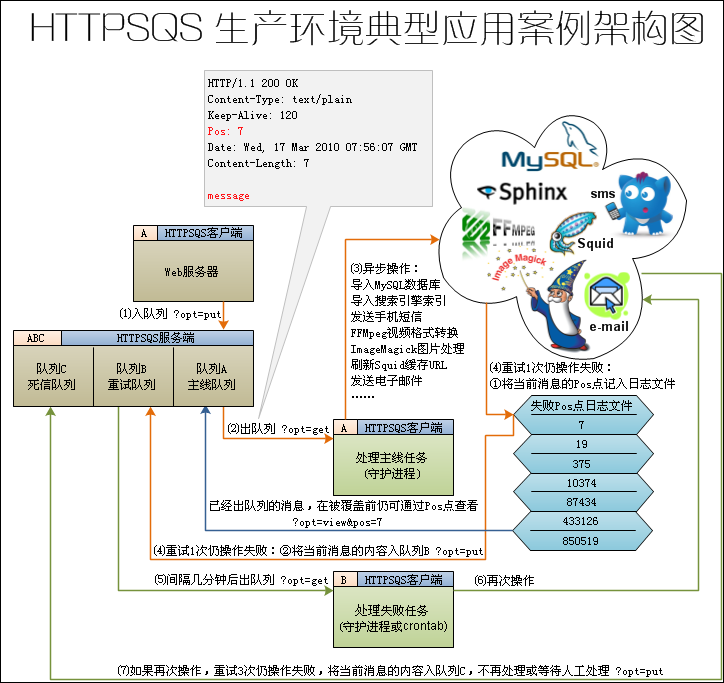
\includegraphics[scale=0.3]{httpsqs_error_handling.png}
\caption{HTTPSQS 生产环境典型应用案例架构}
\end{figure}


一个采用PHP编写的HTTPSQS客户端简单守护进程框架如下:


假设PHP安装路径为/usr/local/webserver/php,使用PHP编写一个文件/opt/httpsqs\_client\_daemon.php:

\begin{lstlisting}[language=bash]
<?php
include_once dirname(__FILE__)."/httpsqs_client.php";   
$httpsqs = new httpsqs($host, $port, $auth, $charset);
while(true) {
  $result = $httpsqs->gets($name);
  $pos = $result["pos"]; //当前队列消息的读取位置点
  $data = $result["data"]; //当前队列消息的内容
  if ($data != "HTTPSQS_GET_END" && $data != "HTTPSQS_ERROR") {
    ...去做应用操作...
  } else {
    sleep(1); //暂停1秒钟后,再次循环
  }
}
\end{lstlisting}

在Linux下,推送到后台执行即可:







\begin{lstlisting}[language=bash]
# nohup /usr/local/webserver/php/bin/php /opt/httpsqs_client_daemon.php 2>&1 > /dev/null &
\end{lstlisting}



\chapter{ZeroMQ}


ZeroMQ是一个为可伸缩的分布式或并发应用程序设计的高性能异步消息库。

ZeroMQ提供一个消息队列, 但是与面向消息的中间件不同,ZeroMQ的运行不需要专门的消息代理(message broker),该库提供了常见的套接字风格的API。

ZeroMQ类库提供一些套接字(对传统Berkeley套接字和Unix domain socket的泛化),每一个套接字可以代表一个端口之间的多对多连接。以消息的粒度进行操作,套接字需要使用一种消息模式(message pattern),然后专门为那种模式进行了优化。


基本的ZeroMQ模式有:

\begin{compactitem}
\item 请求响应模式 - 将一组客户端连接到一组服务器。这是一种远程过程调用和任务分发模式。


\item 发布/订阅模式 - 将一组发布者连接到一组订阅者。这是一种数据分发模式。


\item 管道模式 - 以扇出/扇入模式连接节点,可以有多个步骤,可以有循环。这是一种并行的任务分发和收集模式。


\item 排他对模式 - 在一个排他对中连接两个套接字。 (这是一种高级的为某种用例而设计的低级别模式)

\end{compactitem}

任何通过套接字的消息被看作不透明的数据块。发送给订阅者的消息可以自动地通过块最开始的字符串进行过滤。ZeroMQ提供多种消息传输协议,包括TCP,PGM(可靠的多播),进程间通信(IPC) 以及线程间通讯(ITC)。

由于内部线程模型,ZeroMQ的性能非常好,通过利用一种自动消息批处理技术,它甚至在吞吐量上超过了TCP的性能。

ZeroMQ实现了ZMTP, ZeroMQ消息传输协议。

ZMTP定义了向后兼容性的规则,可扩展的安全机制,命令和消息分帧,连接元数据,以及其他传输层功能。不使用完整的ZeroMQ实现,而是直接实现ZMTP协议的项目不断增加。


\chapter{STOMP}


PHP的Stomp扩展可以让PHP应用和任何Stomp兼容的Message Broker通信,而且Stomp扩展支持面向对象和过程式的接口语法。

\section{Requirement}


PECL/Stomp需要OpenSSL、PECL/openssl的支持才能进行SSL加密通信。






